
\subsection{Skyline Computation}

Techniques of the computation of skyline records in traditional
database systems have been studied
in~\cite{conf/icde/BorzsonyiKS01,shooting_stars,progressive_skyline}.
The well-known algorithms are Nest-Loop, Block-Nested-Loop, and
Divide and Conquer. The Nest-Loop algorithm is an intuitive way to
compute skyline points in the way that every record is compared
with every other record in a table to determine if the record is
dominated. In Block-Nested-Loop, a record is only compared with
other records in the same block. The candidate skyline points in
each block are compared to obtain the final skyline points. In
Divide and Conquer (D\&C), the data set is recursively divided
until there are only two records. Skyline points are calculated
for each segment produced in the division phase. The division
phase is followed by a merge phase in which the skyline of all
divisions are compared and merged to obtain the final skyline set.

\cite{shooting_stars} introduces an online skyline computation
algorithm in which the skyline are computed progressively. The
first skyline is returned almost immediately and more skyline
points are added to the result set.

Nearest Neighbor (NN) and Branch-and-Bound (BBS) skyline
algorithms are two of the best-performing algorithms for
progressive skyline computation for traditional database systems
presented in~\cite{progressive_skyline}. In the NN skyline
algorithm, the records of the data set are presented geometrically
in a Euclidean space with the relevant attributes as the
coordinate in each dimension. In the example of a hotel close to
the ocean previously presented, a record would be placed on a
plane with the distance of the hotel to the ocean and its price as
the two axes that determine its ranking, and the values in the two
attributes as the coordinates of the records on the Euclidean
plane. The NN algorithm finds a nearest neighbor from the axes;
that is the first skyline point. Then the algorithm marks the
region that is dominated by the first skyline point so that
anything in that region will not be searched. The search results
in two more search regions and the search continues until no more
records are left.

%as in Figure~\ref{fig:skyline_nn}

%\begin{figure}[h]
%\begin{center}
%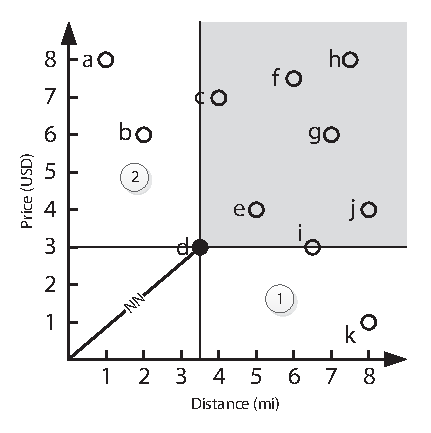
\includegraphics[width=2in]{Figures/skyline_nn.eps}
%\vspace*{-5pt} \caption{NN d and its pruning region.}
%\label{fig:skyline_nn} \vspace*{-10pt}
%\end{center}
%\end{figure}

BBS is an algorithm that surpasses the computation efficiency of
the NN algorithm. BBS utilizes the best first search technique to
traverse the index tree to prune the unnecessary branches.
Unfortunately, both NN and BBS cannot be easily adopted to the
broadcast environment due to the linear nature of the broadcast
program. Both NN and BBS require backtracking of the index tree to
find the best path to prune (which is impermissible in the
broadcast environment) or require waiting for the next broadcast
cycle (which incurs a long waiting time). The solutions presented
in this paper will use the pruning region strategy used in NN. Our
algorithms systematically build pruning regions, as presented in
the NN algorithm, as the client receives and discovers more data
from the broadcast channel.

% SQL Operator
Extension SQL syntax for skyline was defined by B{\"o}rzs{\"o}nyi
et al. in~\cite{conf/icde/BorzsonyiKS01}. The syntax defines an
additional SKYLINE clause in SQL that specifies how the skyline
operation should be performed. In the SKYLINE clause, relevant
attributes can be listed. For each attribute, the syntax defines
three attribute specifiers, MIN, MAX, and DIFF, that tell the
operator how each attribute is to be handled. MIN and MAX denote
that the values of the attribute should be minimized or maximized;
DIFF denotes that the values should be different.

\subsection{Wireless Broadcast Index}\label{sec:wireless_bcast_index}

Many excellent studies have been done on improving the efficiency
of wireless broadcast systems using indexing techniques. This
section considers several popular index allocation techniques and
discusses their benefits and drawbacks.

The intuitive technique of no index and one-time index at the
beginning of a broadcast cycle has been considered
in~\cite{journals/tkde/ImielinskiVB97}. With no index, the length
of a cycle is minimized, but the tuning time is the entire cycle
since the program is not self-descriptive. With one-time index,
the clients are able to filter unwanted data and reduce tuning
time, but if a client misses the one-time index, then it will have
to wait until the next cycle even if there is useful data in
current cycle.

$(1, m)$ indexing, proposed by Imielinski, \emph{et al.}
in~\cite{journals/tkde/ImielinskiVB97}, is a mitigation to the
problem of one-time index by replicating the entire index every
$1/m$ length of the broadcast cycle. The benefit of this index
technique is that when a client misses an index segment, it can
wait for the next index in the same
cycle~\cite{journals/tmc/KuZW08}. The drawback of this technique
is the space consumption of replicating the full index several
times in the cycle.

Distributed index was also proposed
in~\cite{journals/tkde/ImielinskiVB97}. This index also replicates
the index in the broadcast cycle, but only a part of the index is
replicated. Advantages of this method are (1) an index can be
obtained throughout a cycle, (2) reduced bandwidth consumption
compared with $(1, m)$, and (3) the method is not limited to any
particular index structure.

%\cite{data_on_air} by Imielinski, et al. is an
%early and influential work of data
%indexing for broadcast on air. The paper defined two
%characteristics of wireless broadcast, \em{tuning time} and \em{access latency}. Tuning time
%defines how long the client has to actively listen on the channel to get all the desired data.
%Access latency define the time when the client issues the query to the time all the desired
%data is received. Tuning time is proportional to power usage of mobile clients. The goal is to
%reduce both tuning time and access latency.

%In addition, the paper also proposed a few air index techniques to reduce client tuning time.
%The first index proposed is $(1, m)$ index, in which the full index is repeated every $1/m$ of
%the entire broadcast cycle. The index is repeat so that clients that tune into the channel in
%the middle of the broadcast does not have to wait until the next cycle to get the index and
%process request. The second index proposed is the distributed index, in which only a part of
%the index is repeated. Distributed index reduces the overhead of embedding index and improves
%access latency.

Data filtering based on data signatures was proposed
in~\cite{journals/winet/LeeL99}. During data retrieval, the
signature of the desired data is compared with the signature of a
data segment prepared by the broadcast server. If the signatures
match, then the data is downloaded; otherwise it is ignored.

Distributed index for spatial data in error-prone air broadcast
was introduced in~\cite{journals/vldb/ZhengLLLS09}. Instead of
replication, this paper proposes a distributed index in the
broadcast cycle with no duplicate indexes. The paper indexes
broadcast spatial data using Hilbert values. Each data record
contains an index table that includes the data segments that will
be pushed onto the channel in the near future. A drawback of this
approach is the loss of spatial precision due to the use of the
space filling curve as the index.


%\section{System Model}

%In our theoretical model, the system consists of the broadcast server and multiple clients. As
%discussed in section 2.1, the server periodically broadcast data in a specific channel. Any client
%that is interested in any of the data serviced by the server tunes into the channel to get the
%desire data. The server contains a set of records as illustrated in Figure 4.

%In this model, we assume a pure broadcast model in which all data are transmitted through downlink
%bandwidth and that there is not uplink bandwidth. Clients must tune into the channel as long as it
%takes to obtain all desire data. Apparently, in order to support efficient query, the server must
%provide data index so that the client can tune in only when the relevant data is to be broadcasted
%In addition, this model contains only one transmission channel. Index must be transmitted on the
%same channel as the data.
